% orthoresponse user manual -- compile with:  latexmk -xelatex orthoresponse_manual.tex
\documentclass[11pt,a4paper]{article}

% ------------------------------------------------------------------ layout
\usepackage[a4paper, top=24mm, bottom=24mm, left=24mm, right=24mm, headheight=14pt]{geometry}
\usepackage{fontspec}
\setmainfont{ManualSerif}[Path=fonts/, Extension=.ttf, UprightFont=*-Regular, BoldFont=*-Bold,
  ItalicFont=*-Italic, BoldItalicFont=*-BoldItalic, Scale=0.9]
\setsansfont{Inter}[Scale=0.92]
\setmonofont{DejaVu Sans Mono}[Scale=0.80]
\usepackage{unicode-math}
\setmathfont{Latin Modern Math}
\usepackage{microtype}
\usepackage[dvipsnames,svgnames]{xcolor}
\usepackage{graphicx}
\usepackage{booktabs, tabularx, array, multirow}
\usepackage{enumitem}
\usepackage{titlesec}
\usepackage{fancyhdr}
\usepackage{caption}
\usepackage{float}
\usepackage[section]{placeins}
\usepackage[most]{tcolorbox}
\usepackage{listings}
\usepackage{tikz}
\usetikzlibrary{arrows.meta, positioning, calc, shapes.geometric, shadows.blur, fit, backgrounds}
\usepackage[edges]{forest}
\usepackage{hyperref}

% ------------------------------------------------------------------ colours
\definecolor{navy}{HTML}{2F4B8A}
\definecolor{navylight}{HTML}{E9EEF8}
\definecolor{grpA}{HTML}{1F77B4}
\definecolor{grpB}{HTML}{FF7F0E}
\definecolor{ink}{HTML}{1E2433}
\definecolor{muted}{HTML}{6B7385}
\definecolor{codebg}{HTML}{F6F8FB}
\definecolor{termbg}{HTML}{1E2230}
\definecolor{termfg}{HTML}{E6E9F0}
\definecolor{okgreen}{HTML}{2E8B57}
\definecolor{warnred}{HTML}{C0392B}
\definecolor{tipamber}{HTML}{B7791F}

\hypersetup{colorlinks=true, linkcolor=navy, urlcolor=navy, citecolor=navy,
  pdftitle={orthoresponse user manual}, pdfauthor={J. Sebastián Contreras-Riquelme}}

\color{ink}
\setlength{\parindent}{0pt}
\setlength{\parskip}{5pt}
\linespread{1.08}
\setlist{itemsep=2pt, topsep=3pt}

% ------------------------------------------------------------------ headings
\titleformat{\section}{\sffamily\Large\bfseries\color{navy}}{\thesection}{0.8em}{}[{\color{navy}\titlerule[0.8pt]}]
\titleformat{\subsection}{\sffamily\large\bfseries\color{ink}}{\thesubsection}{0.7em}{}
\titleformat{\subsubsection}{\sffamily\normalsize\bfseries\color{navy}}{}{0em}{}
\titlespacing*{\section}{0pt}{16pt}{8pt}
\titlespacing*{\subsection}{0pt}{12pt}{4pt}
\captionsetup{font={small,sf}, labelfont={bf,color=navy}, margin=4pt}

\pagestyle{fancy}
\fancyhf{}
\fancyhead[L]{\sffamily\footnotesize\color{muted} orthoresponse \textbullet{} User manual}
\fancyhead[R]{\sffamily\footnotesize\color{muted} \nouppercase{\leftmark}}
\fancyfoot[C]{\sffamily\footnotesize\color{muted}\thepage}
\renewcommand{\headrulewidth}{0.4pt}
\renewcommand{\headrule}{{\color{navylight}\hrule height 0.8pt}}
\renewcommand{\sectionmark}[1]{\markboth{#1}{}}

% ------------------------------------------------------------------ code
\lstdefinestyle{base}{
  basicstyle=\ttfamily\small\color{ink}, columns=fullflexible, keepspaces=true,
  keywordstyle=\color{navy}\bfseries, stringstyle=\color{okgreen!80!black},
  commentstyle=\color{muted}\itshape, showstringspaces=false, breaklines=true,
  upquote=true}
\lstdefinestyle{py}{style=base, language=Python,
  morekeywords={True,False,None}}
\lstdefinestyle{r}{style=base, language=R, morekeywords={library,TRUE,FALSE,NULL}, deletekeywords={save,data,list,c}}
\lstdefinestyle{sh}{style=base, language=bash, morekeywords={pip,git,orthoresponse,Rscript,python,blastp,makeblastdb,cd}}
\lstdefinestyle{plain}{style=base, keywordstyle=\color{ink}}

\newtcblisting{pycode}{enhanced, colback=codebg, colframe=grpA!55, boxrule=0.5pt, arc=3pt,
  left=6pt, right=6pt, top=3pt, bottom=3pt, listing only, listing options={style=py},
  borderline west={2.5pt}{0pt}{grpA}, attach boxed title to top right={xshift=-4pt, yshift=-8pt},
  title={\sffamily\scriptsize\bfseries Python}, coltitle=white, colbacktitle=grpA,
  boxed title style={arc=2pt, boxrule=0pt}}
\newtcblisting{rcode}{enhanced, colback=codebg, colframe=grpB!60, boxrule=0.5pt, arc=3pt,
  left=6pt, right=6pt, top=3pt, bottom=3pt, listing only, listing options={style=r},
  borderline west={2.5pt}{0pt}{grpB}, attach boxed title to top right={xshift=-4pt, yshift=-8pt},
  title={\sffamily\scriptsize\bfseries R}, coltitle=white, colbacktitle=grpB,
  boxed title style={arc=2pt, boxrule=0pt}}
\newtcblisting{shcode}{enhanced, colback=codebg, colframe=muted!50, boxrule=0.5pt, arc=3pt,
  left=6pt, right=6pt, top=3pt, bottom=3pt, listing only, listing options={style=sh},
  borderline west={2.5pt}{0pt}{muted}, attach boxed title to top right={xshift=-4pt, yshift=-8pt},
  title={\sffamily\scriptsize\bfseries Shell}, coltitle=white, colbacktitle=muted,
  boxed title style={arc=2pt, boxrule=0pt}}
\newtcblisting{plaincode}{enhanced, colback=codebg, colframe=muted!40, boxrule=0.5pt, arc=3pt,
  left=6pt, right=6pt, top=3pt, bottom=3pt, listing only, listing options={style=plain}}
% terminal mockup
\newtcblisting{terminal}[1]{enhanced, colback=termbg, colframe=termbg, arc=5pt, boxrule=0pt,
  left=8pt, right=8pt, top=20pt, bottom=6pt, listing only,
  listing options={basicstyle=\ttfamily\scriptsize\color{termfg}, columns=fullflexible, keepspaces=true, breaklines=false},
  overlay={
    \fill[termbg!70!white] ([yshift=-16pt]frame.north west) rectangle (frame.north east);
    \fill[termbg!70!white, rounded corners=5pt] (frame.north west) rectangle ([yshift=-16pt]frame.north east);
    \fill[red!70]    ([xshift=12pt, yshift=-8pt]frame.north west) circle (3pt);
    \fill[orange!80] ([xshift=23pt, yshift=-8pt]frame.north west) circle (3pt);
    \fill[green!60!black] ([xshift=34pt, yshift=-8pt]frame.north west) circle (3pt);
    \node[font=\sffamily\scriptsize, text=termfg!80] at ([yshift=-8pt]frame.north) {#1};}}

% callouts
\newtcolorbox{note}[1][Note]{enhanced, colback=navylight, colframe=navy, boxrule=0pt, arc=3pt,
  borderline west={3pt}{0pt}{navy}, left=8pt, fonttitle=\sffamily\bfseries\small, coltitle=navy,
  colbacktitle=navylight, title={#1}, attach title to upper={\enspace}, fontupper=\small}
\newtcolorbox{caution}[1][Caution]{enhanced, colback=red!4, colframe=warnred, boxrule=0pt, arc=3pt,
  borderline west={3pt}{0pt}{warnred}, left=8pt, fonttitle=\sffamily\bfseries\small, coltitle=warnred,
  title={#1}, attach title to upper={\enspace}, fontupper=\small}
\newtcolorbox{tip}[1][Tip]{enhanced, colback=orange!5, colframe=tipamber, boxrule=0pt, arc=3pt,
  borderline west={3pt}{0pt}{tipamber}, left=8pt, fonttitle=\sffamily\bfseries\small, coltitle=tipamber,
  title={#1}, attach title to upper={\enspace}, fontupper=\small}

\newcommand{\code}[1]{\texttt{\color{navy!85!black}#1}}
\newcommand{\pkg}{\textsf{\bfseries orthoresponse}}
\newcommand{\A}{\textcolor{grpA}{\textbf{A}}}
\newcommand{\B}{\textcolor{grpB}{\textbf{B}}}
\newcolumntype{Y}{>{\raggedright\arraybackslash}X}
\renewcommand{\arraystretch}{1.18}

% ------------------------------------------------------------------ tikz styles
\tikzset{
  cell/.style={draw, rounded corners=4pt, minimum width=3.3cm, minimum height=1.45cm, align=center,
               font=\sffamily\small, line width=0.8pt, blur shadow={shadow blur steps=4, shadow xshift=0.6pt, shadow yshift=-0.8pt}},
  ctr/.style={-{Stealth[length=2.6mm]}, line width=1pt, navy},
  clab/.style={font=\sffamily\scriptsize, fill=white, inner sep=1.5pt, text=navy},
  flow/.style={draw=navy, fill=navylight, rounded corners=4pt, align=center, font=\sffamily\small,
               minimum height=1.35cm, text width=2.55cm, line width=0.7pt},
  flowarrow/.style={-{Stealth[length=2.6mm]}, line width=1pt, navy},
}

% mini pattern glyph used on the cover: #1 = A control, #2 = A stress, #3 = B control, #4 = B stress
\newcommand{\glyph}[4]{%
  \begin{tikzpicture}[x=0.36cm, y=0.32cm]
    \draw[white, opacity=0.25, rounded corners=2pt] (-0.3,-1.6) rectangle (6.3,1.6);
    \draw[white, opacity=0.35, dashed] (3,-1.4) -- (3,1.4);
    \draw[grpA!45!white, line width=1.6pt, line cap=round] (0,#1) -- (1,#1) -- (2,#2) -- (3,#2);
    \draw[grpB!80!white, line width=1.6pt, line cap=round] (3,#3) -- (4,#3) -- (5,#4) -- (6,#4);
  \end{tikzpicture}}

\begin{document}

% ================================================================== COVER
\begin{titlepage}
\newgeometry{margin=0pt}

\begin{tikzpicture}[remember picture, overlay]
  \fill[navy] (current page.north west) rectangle ([yshift=-15.5cm]current page.north east);
  \fill[navy!85!black] ([yshift=-15.5cm]current page.north west) rectangle ([yshift=-16.1cm]current page.north east);
  \node[anchor=north west, text=white, font=\sffamily\bfseries\fontsize{40}{44}\selectfont]
    at ([xshift=2.4cm, yshift=-3.1cm]current page.north west) {orthoresponse};
  \node[anchor=north west, text=white, text width=15cm, font=\sffamily\Large]
    at ([xshift=2.45cm, yshift=-4.85cm]current page.north west)
    {Expression response models of orthologs and genes\\in two-by-two designs};
  \node[anchor=north west, text=white!80, font=\sffamily\normalsize]
    at ([xshift=2.45cm, yshift=-6.65cm]current page.north west)
    {User manual \quad\textbullet\quad Version 0.4.1 \quad\textbullet\quad Python and R};
  % pattern glyphs
  \node[anchor=north west] at ([xshift=2.3cm, yshift=-8.6cm]current page.north west) {%
    \begin{tabular}{@{}c@{\hspace{5mm}}c@{\hspace{5mm}}c@{\hspace{5mm}}c@{\hspace{5mm}}c@{}}
      \glyph{0}{1}{1}{1} & \glyph{0}{1}{0}{1} & \glyph{0}{1}{0}{0} & \glyph{0}{1}{0}{-1} & \glyph{0}{0}{1}{1}\\[2pt]
      \textcolor{white}{\sffamily\scriptsize stress-ready} & \textcolor{white}{\sffamily\scriptsize shared} &
      \textcolor{white}{\sffamily\scriptsize unique} & \textcolor{white}{\sffamily\scriptsize opposite} &
      \textcolor{white}{\sffamily\scriptsize no response}
    \end{tabular}};
  \node[anchor=north west, text=white!85, text width=16.5cm, font=\sffamily\small]
    at ([xshift=2.45cm, yshift=-12.1cm]current page.north west)
    {Two groups (species, genotypes, cultivars or cell lines) \(\times\) two conditions (control and stress).
     For every gene or ortholog pair: does one group already express, without stress, what the other
     only reaches under stress?};
  % lower part
  \node[anchor=north west, text width=16.5cm, font=\sffamily\small, text=ink]
    at ([xshift=2.45cm, yshift=-17.6cm]current page.north west) {%
    \textbf{\color{navy}What you will find in this manual}\\[4pt]
    \begin{tabular}{@{}p{7.6cm}p{7.6cm}@{}}
      \textbullet\ What the five response models mean & \textbullet\ Options, presets and their effect\\
      \textbullet\ How the decision tree works & \textbullet\ Every output file and figure\\
      \textbullet\ Installation in Python and R & \textbullet\ Two worked examples with real data\\
      \textbullet\ Quick start with bundled data & \textbullet\ Cross-species analyses with orthologs\\
      \textbullet\ Input formats and templates & \textbullet\ Interpretation caveats and troubleshooting
    \end{tabular}};
  \node[anchor=south west, text=muted, font=\sffamily\small, text width=16.5cm]
    at ([xshift=2.45cm, yshift=2.2cm]current page.south west)
    {J. Sebastián Contreras-Riquelme\\
     \href{https://github.com/Cold7/orthoresponse}{github.com/Cold7/orthoresponse} \quad\textbullet\quad MIT license \quad\textbullet\quad November 2026};
\end{tikzpicture}
\restoregeometry
\end{titlepage}

% ================================================================== TOC
\pagenumbering{roman}
\setcounter{tocdepth}{2}
{\hypersetup{linkcolor=ink}\sffamily\small\setlength{\parskip}{0pt}\tableofcontents}
\clearpage
\pagenumbering{arabic}

% ================================================================== 1
\section{What is orthoresponse?}

\pkg{} is a Python and R package that compares how \emph{two groups} respond to \emph{the same
stress}. The groups can be two species (compared through their orthologous genes), two genotypes
or cultivars of one species, or two cell lines. Each group is measured under a \textbf{control}
and a \textbf{stress} condition, so the experiment is a \(2\times2\) design.

For every gene, or every pair of orthologs, the package decides which of five \emph{expression
response models} describes the data best:

\begin{center}
\begin{tabularx}{0.94\linewidth}{>{\sffamily\bfseries}l Y}
\toprule
\textcolor{navy}{stress-ready} & one group responds, and under stress it reaches the level that the
other group already has \emph{without} stress. The other group is \emph{primed}.\\
\textcolor{navy}{shared} & both groups respond in the same direction.\\
\textcolor{navy}{unique} & only one group responds.\\
\textcolor{navy}{opposite} & both groups respond, in opposite directions.\\
\textcolor{navy}{no response} & neither group responds (the basal levels may still differ).\\
\bottomrule
\end{tabularx}
\end{center}

The idea of a \emph{stress-ready} (or pre-adapted) transcriptome comes from comparisons between
stress-sensitive plants and their stress-tolerant relatives, where the tolerant species
constitutively express genes that the sensitive species only induce under stress. With its default
settings \pkg{} reproduces exactly the decision tree used by Contreras-Riquelme \emph{et al.}
(2025, \emph{PLoS One} 20(5): e0324724) to compare cultivated tomato and the desert-adapted
\emph{Solanum pennellii} under drought, and adds stricter, optional rules.

\subsection{Key features}
\begin{itemize}
  \item \textbf{One call from counts to answers}: a single DESeq2 (R) or PyDESeq2 (Python) fit, five
        contrasts, classification, summaries and figures.
  \item \textbf{Two presets}: \code{paper} (the published rules) and \code{strict} (handles missing
        statistics and requires a basal difference for stress-ready calls), plus an optional formal
        equivalence test.
  \item \textbf{Identical in Python and R}: same function names, options and outputs; both
        implementations give the same label for every feature given the same contrasts.
  \item \textbf{Cross-species support}: reciprocal best BLAST hits and ortholog-level count matrices.
  \item \textbf{Real example data included}: rice under salt stress and human ovarian cancer cells
        under a metabolic drug, ready to run.
  \item \textbf{Publication-ready figures} saved automatically (PNG and PDF), with configurable labels.
\end{itemize}

\subsection{When to use it}
Use \pkg{} when you have RNA-seq raw counts for a complete \(2\times2\) design and want to know
whether one group is \emph{pre-adapted} to a stress, which responses are conserved, and which are
group-specific. Typical questions:
\begin{itemize}
  \item Does a drought-tolerant wild relative constitutively express genes that the crop only induces under drought?
  \item Does a drug-resistant cell line already express what the sensitive line induces under the drug?
  \item Which stress responses are shared by two cultivars, and which are unique to the tolerant one?
\end{itemize}

% ================================================================== 2
\section{Concepts}

\subsection{The two-by-two design}

Every analysis is built on four groups of samples and five pairwise comparisons
(Figure~\ref{fig:design}). Group \A{} is the \emph{reference}, usually the sensitive group; group
\B{} is the \emph{comparison}, usually the tolerant or adapted one. Which group you call \A{} only
changes the case numbers, never the biology.

\begin{figure}[htbp]
\centering
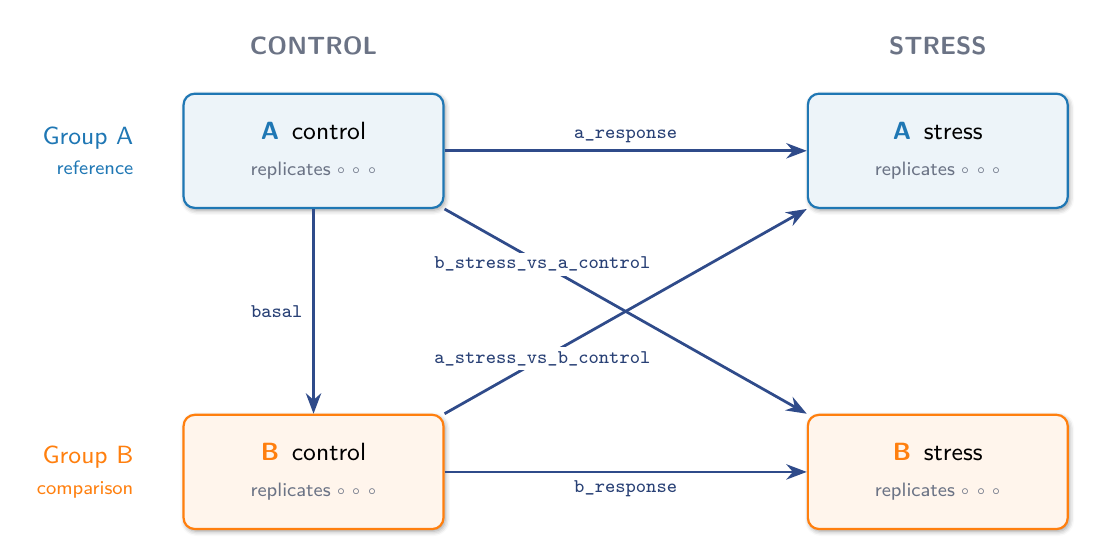
\begin{tikzpicture}[node distance=1.2cm and 3.3cm]
  \node[cell, draw=grpA, fill=grpA!8] (ac) {\textbf{\textcolor{grpA}{A}} \,control\\[2pt]\scriptsize\color{muted} replicates \(\circ\,\circ\,\circ\)};
  \node[cell, draw=grpA, fill=grpA!8, right=4.6cm of ac] (as) {\textbf{\textcolor{grpA}{A}} \,stress\\[2pt]\scriptsize\color{muted} replicates \(\circ\,\circ\,\circ\)};
  \node[cell, draw=grpB, fill=grpB!8, below=2.6cm of ac] (bc) {\textbf{\textcolor{grpB}{B}} \,control\\[2pt]\scriptsize\color{muted} replicates \(\circ\,\circ\,\circ\)};
  \node[cell, draw=grpB, fill=grpB!8, below=2.6cm of as] (bs) {\textbf{\textcolor{grpB}{B}} \,stress\\[2pt]\scriptsize\color{muted} replicates \(\circ\,\circ\,\circ\)};
  \draw[ctr] (ac) -- node[clab, above=1pt] {\code{a\_response}} (as);
  \draw[ctr] (bc) -- node[clab, below=1pt] {\code{b\_response}} (bs);
  \draw[ctr] (ac) -- node[clab, left=2pt] {\code{basal}} (bc);
  \draw[ctr] (ac.south east) -- node[clab, pos=0.27] {\code{b\_stress\_vs\_a\_control}} (bs.north west);
  \draw[ctr] (bc.north east) -- node[clab, pos=0.27] {\code{a\_stress\_vs\_b\_control}} (as.south west);
  \node[font=\sffamily\small\bfseries, text=muted, above=0.35cm of ac] {CONTROL};
  \node[font=\sffamily\small\bfseries, text=muted, above=0.35cm of as] {STRESS};
  \node[font=\sffamily\small, text=grpA, left=0.5cm of ac, align=right] {Group A\\\scriptsize reference};
  \node[font=\sffamily\small, text=grpB, left=0.5cm of bc, align=right] {Group B\\\scriptsize comparison};
\end{tikzpicture}
\caption{The \(2\times2\) design and the five contrasts used by the classifier. Each arrow points from the
denominator to the numerator: a positive log2 fold change means \emph{higher at the arrow head}.}
\label{fig:design}
\end{figure}

\subsection{The fifteen patterns}

The five models split into fifteen cases according to the direction of the change
(Figure~\ref{fig:patterns}, Table~\ref{tab:models}). In every panel the left half shows group \A{}
and the right half group \B{}; within each half, control is on the left and stress on the right.

\begin{figure}[htbp]
\centering
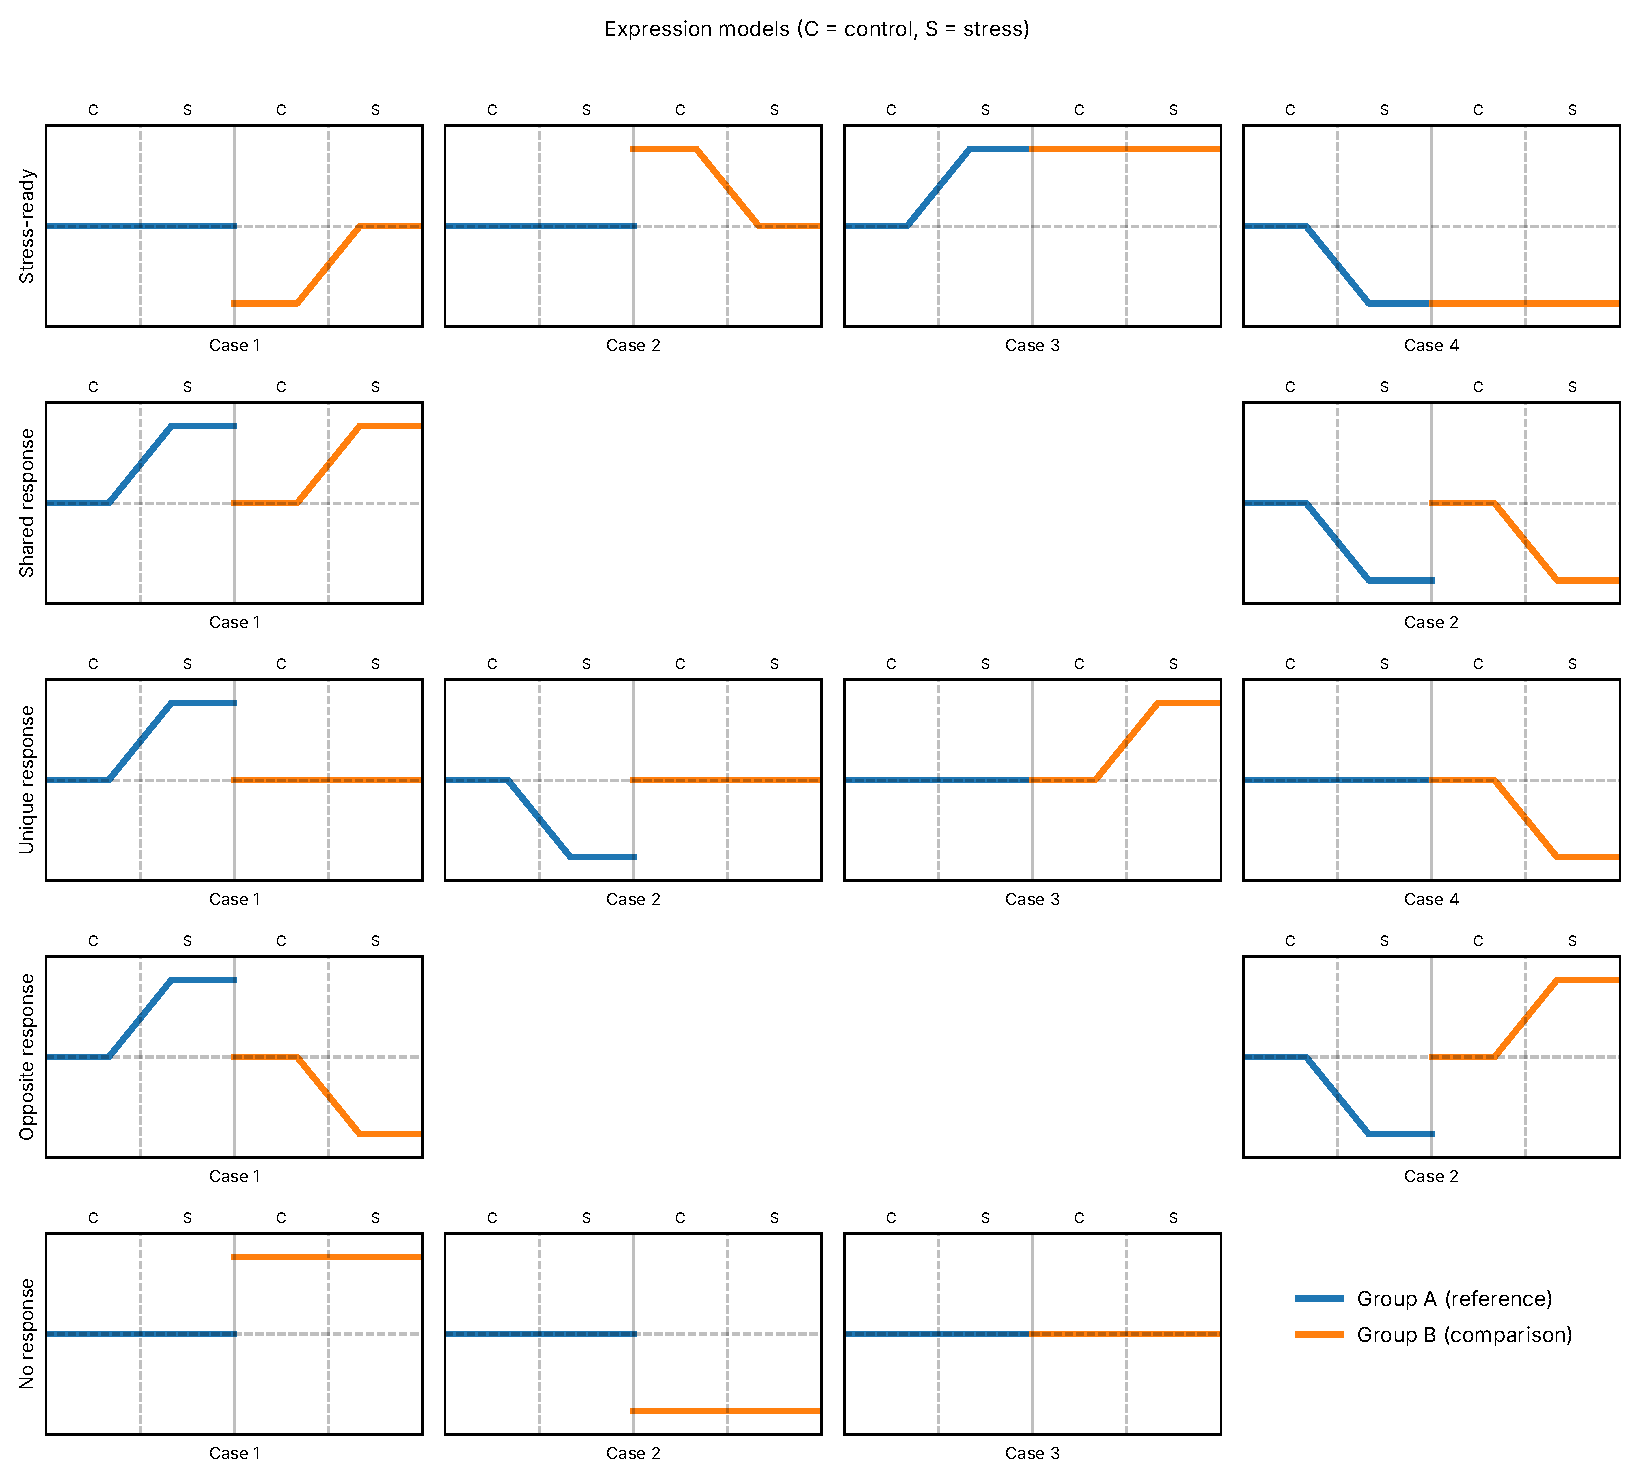
\includegraphics[width=0.93\linewidth]{figures/patterns_generic.pdf}
\caption{Schematic of the fifteen expression patterns (C = control, S = stress). Shared and opposite
responses are drawn in the outer columns.}
\label{fig:patterns}
\end{figure}

\begin{table}[htbp]
\centering\small
\caption{Labels produced by the classifier. The \emph{primed} group is the one whose control level equals
the other group's stressed level.}
\label{tab:models}
\begin{tabularx}{\linewidth}{>{\ttfamily\color{navy!85!black}}l Y c}
\toprule
\textsf{\textbf{label}} & \textsf{\textbf{meaning}} & \textsf{\textbf{primed}}\\
\midrule
stress\_ready\_1 & B is induced under stress up to the control level of A & \A\\
stress\_ready\_2 & B is repressed under stress down to the control level of A & \A\\
stress\_ready\_3 & A is induced under stress up to the control level of B & \B\\
stress\_ready\_4 & A is repressed under stress down to the control level of B & \B\\
\midrule
shared\_1 / \_2 & induced / repressed in both groups & --\\
unique\_1 / \_2 & induced / repressed only in A & --\\
unique\_3 / \_4 & induced / repressed only in B & --\\
opposite\_1 / \_2 & induced in A and repressed in B / the reverse & --\\
no\_response\_1 / \_2 & no response; basal level higher / lower in B than in A & --\\
no\_response\_3 & no response; no basal difference detected & --\\
\midrule
unresolved\_\(k\) & only with an equivalence test: neither different nor equivalent & --\\
unclassified & only with \code{na\_action="unclassified"}: missing statistics & --\\
\bottomrule
\end{tabularx}
\end{table}

\begin{note}[In short]
Stress-ready cases 1--2 mean that \A{} is primed; cases 3--4 mean that \B{} is primed. If \B{} is your
tolerant group, cases 3 and 4 are the ones that support pre-adaptation of \B.
\end{note}

% ================================================================== 3
\section{How it works}

\subsection{The workflow}

\begin{figure}[htbp]
\centering
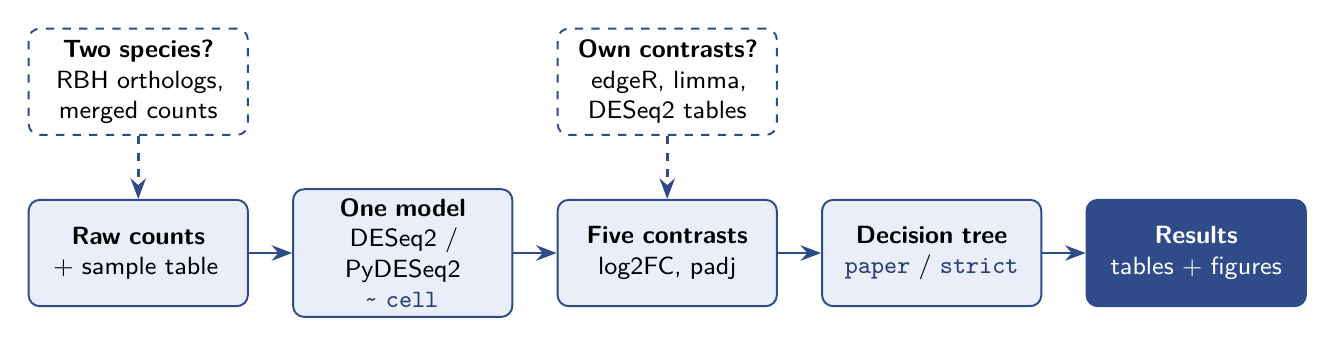
\begin{tikzpicture}[node distance=0.55cm]
  \node[flow] (in) {\textbf{Raw counts}\\+ sample table};
  \node[flow, right=of in] (fit) {\textbf{One model}\\DESeq2 / PyDESeq2\\\code{\textasciitilde{} cell}};
  \node[flow, right=of fit] (ct) {\textbf{Five contrasts}\\log2FC, padj};
  \node[flow, right=of ct] (tree) {\textbf{Decision tree}\\\code{paper} / \code{strict}};
  \node[flow, right=of tree, fill=navy, text=white] (out) {\textbf{Results}\\tables + figures};
  \foreach \a/\b in {in/fit, fit/ct, ct/tree, tree/out} \draw[flowarrow] (\a) -- (\b);
  \node[flow, above=0.8cm of in, fill=white, dashed] (orth) {\textbf{Two species?}\\RBH orthologs,\\merged counts};
  \draw[flowarrow, dashed] (orth) -- (in);
  \node[flow, above=0.8cm of ct, fill=white, dashed] (own) {\textbf{Own contrasts?}\\edgeR, limma,\\DESeq2 tables};
  \draw[flowarrow, dashed] (own) -- (ct);
\end{tikzpicture}
\caption{From counts to classification. Dashed boxes are optional entry points.}
\label{fig:workflow}
\end{figure}

\begin{enumerate}
  \item \textbf{Design.} Samples are mapped to four cells: \code{A\_control}, \code{A\_stress},
        \code{B\_control}, \code{B\_stress}.
  \item \textbf{Filtering.} Features with a total count \(\le\) \code{min\_total\_count} (default 10)
        are removed.
  \item \textbf{Model.} One negative-binomial model is fitted to all samples with the design
        \code{\textasciitilde{} cell}; size factors and dispersions are estimated across both groups.
  \item \textbf{Contrasts.} The five contrasts of Figure~\ref{fig:design} are extracted with
        Benjamini--Hochberg adjustment, Cook's outlier filtering and independent filtering.
  \item \textbf{Classification} with the decision tree below.
  \item \textbf{Summaries and figures}: counts per model with explicit denominators, the
        primed-asymmetry test, and the figures of Section~\ref{sec:outputs}.
\end{enumerate}

\subsection{The decision tree}

A contrast is \emph{significant} when its adjusted p-value is below \code{alpha} (default 0.05) and,
optionally, \(|\log_2\mathrm{FC}|\) is at least \code{min\_abs\_lfc}. Its \emph{direction} is the sign of
the log2 fold change.

\begin{figure}[htbp]
\centering
\resizebox{\linewidth}{!}{%
\begin{forest}
  for tree={draw=navy, rounded corners=3pt, fill=navylight, align=center, font=\sffamily\scriptsize,
            inner sep=3pt, l sep=7mm, s sep=2.2mm, edge={navy, line width=0.7pt}, parent anchor=south,
            child anchor=north}
  [{\textbf{Does A respond?}\\\code{a\_response}}
    [{\textbf{Does B respond?}\\\code{b\_response}}, edge label={node[midway, left, font=\sffamily\scriptsize\bfseries, fill=white, inner sep=1pt, text=warnred]{no}}
      [{\textbf{Basal difference?}\\\code{basal}}, edge label={node[midway, left, font=\sffamily\scriptsize\bfseries, fill=white, inner sep=1pt, text=warnred]{no}}
        [{no\_response\_1\\(B higher)}, fill=white]
        [{no\_response\_2\\(B lower)}, fill=white]
        [{no\_response\_3\\(none)}, fill=white]]
      [{\textbf{B stress = A control?}\\\code{b\_stress\_vs\_a\_control}}, edge label={node[midway, right, font=\sffamily\scriptsize\bfseries, fill=white, inner sep=1pt, text=okgreen]{yes}}
        [{\textbf{stress\_ready\_1/2}\\(B up / down)}, fill=grpB!15, edge label={node[midway, left, font=\sffamily\scriptsize\bfseries, fill=white, inner sep=1pt, text=okgreen]{yes}}]
        [{unique\_3/4\\(B up / down)}, fill=white, edge label={node[midway, right, font=\sffamily\scriptsize\bfseries, fill=white, inner sep=1pt, text=warnred]{no}}]]]
    [{\textbf{Does B respond?}\\\code{b\_response}}, edge label={node[midway, right, font=\sffamily\scriptsize\bfseries, fill=white, inner sep=1pt, text=okgreen]{yes}}
      [{\textbf{A stress = B control?}\\\code{a\_stress\_vs\_b\_control}}, edge label={node[midway, left, font=\sffamily\scriptsize\bfseries, fill=white, inner sep=1pt, text=warnred]{no}}
        [{\textbf{stress\_ready\_3/4}\\(A up / down)}, fill=grpA!15, edge label={node[midway, left, font=\sffamily\scriptsize\bfseries, fill=white, inner sep=1pt, text=okgreen]{yes}}]
        [{unique\_1/2\\(A up / down)}, fill=white, edge label={node[midway, right, font=\sffamily\scriptsize\bfseries, fill=white, inner sep=1pt, text=warnred]{no}}]]
      [{\textbf{Same direction?}}, edge label={node[midway, right, font=\sffamily\scriptsize\bfseries, fill=white, inner sep=1pt, text=okgreen]{yes}}
        [{shared\_1/2}, fill=white, edge label={node[midway, left, font=\sffamily\scriptsize\bfseries, fill=white, inner sep=1pt, text=okgreen]{yes}}]
        [{opposite\_1/2}, fill=white, edge label={node[midway, right, font=\sffamily\scriptsize\bfseries, fill=white, inner sep=1pt, text=warnred]{no}}]]]]
\end{forest}}
\caption{The decision tree. ``Same level'' (=) means \emph{not significantly different} under the
\code{paper} preset; Section~\ref{sec:options} describes stricter alternatives.}
\label{fig:tree}
\end{figure}

\begin{caution}[Absence of evidence is not evidence of equality]
Under the \code{paper} preset a gene is stress-ready when the responding group's stressed level is
\emph{not significantly different} from the other group's control level. With few replicates this
inflates the stress-ready class. The \code{strict} preset and the equivalence test exist for this
reason; see Sections~\ref{sec:options} and \ref{sec:interpret}.
\end{caution}

% ================================================================== 4
\section{Installation}

\subsection{Python (3.9 or newer)}
\begin{shcode}
# full installation: PyDESeq2, plotting and Excel support
pip install "orthoresponse[all] @ \
  git+https://github.com/Cold7/orthoresponse.git#subdirectory=python"

# a specific version
pip install "orthoresponse[all] @ \
  git+https://github.com/Cold7/orthoresponse.git@v0.4.1#subdirectory=python"

orthoresponse --version
\end{shcode}
Optional extras: \code{deseq} (PyDESeq2), \code{plot} (matplotlib), \code{excel} (openpyxl),
\code{all}, \code{test}. Without extras only the classifier (numpy, pandas, scipy) is installed, which
is enough if you already have contrast tables. Installing from GitHub requires \code{git}.

\subsection{R (4.1 or newer)}
\begin{rcode}
install.packages(c("BiocManager", "remotes"))
BiocManager::install("DESeq2")
remotes::install_github("Cold7/orthoresponse", subdir = "r-package",
                        build_vignettes = TRUE)
library(orthoresponse)
vignette("orthoresponse")
\end{rcode}

% ================================================================== 5
\section{Quick start}

\subsection{Run the bundled example}

The package includes two real data sets (Section~\ref{sec:examples}). This is the fastest way to see
the whole workflow:

\begin{pycode}
import orthoresponse as orr

ex = orr.load_example("rice_salt")            # ex.counts, ex.samples, ex.params
res = orr.run_orthoresponse(ex.counts, ex.samples, **ex.params)
print(res)                                    # summary + asymmetry test
res.save("results")                           # tables + figures
\end{pycode}

\begin{rcode}
library(orthoresponse)
ex  <- load_example("rice_salt")
res <- do.call(orthoresponse, c(list(ex$counts, ex$samples), ex$params))
res                                           # same output as print(res)
save_orthoresponse(res, "results")            # tables + figures
\end{rcode}

Both languages print the same text (shown here for R; Python's \code{print(res)} is identical
in format):

\begin{terminal}{R console}
orthoresponse result: A = PL12 | B = IL22
25045 features classified

          label        model case     n pct_of_responsive pct_of_all
 stress_ready_1 stress_ready    1   281               4.1        1.1
 stress_ready_2 stress_ready    2   407               6.0        1.6
 stress_ready_3 stress_ready    3  1744              25.5        7.0
 stress_ready_4 stress_ready    4  1793              26.2        7.2
       shared_1       shared    1   563               8.2        2.2
       shared_2       shared    2   335               4.9        1.3
       unique_1       unique    1   617               9.0        2.5
       unique_2       unique    2   628               9.2        2.5
       unique_3       unique    3   152               2.2        0.6
       unique_4       unique    4   185               2.7        0.7
     opposite_1     opposite    1    88               1.3        0.4
     opposite_2     opposite    2    41               0.6        0.2
  no_response_1  no_response    1   174                NA        0.7
  no_response_2  no_response    2   196                NA        0.8
  no_response_3  no_response    3 17841                NA       71.2

Stress-ready among single-group responders: PL12-only 74.0%, IL22-only 67.1% (Fisher p = 1.22e-05)
\end{terminal}

\subsection{Run it on your own data}

\begin{pycode}
import pandas as pd
import orthoresponse as orr

counts  = pd.read_csv("counts.tsv",  sep="\t", index_col=0)  # raw counts
samples = pd.read_csv("samples.tsv", sep="\t", index_col=0)  # 1 row/sample

res = orr.run_orthoresponse(
    counts, samples,
    group_col="line", condition_col="treatment",
    group_a="PL12", group_b="IL22",        # A = reference, B = comparison
    control="Control", stress="Salt")
res.save("results", condition_labels=("Ctrl", "NaCl"))
\end{pycode}

\begin{rcode}
counts  <- read.delim("counts.tsv",  row.names = 1, check.names = FALSE)
samples <- read.delim("samples.tsv", row.names = 1)
res <- orthoresponse(counts, samples,
                     group_col = "line", condition_col = "treatment",
                     group_a = "PL12", group_b = "IL22",
                     control = "Control", stress = "Salt")
save_orthoresponse(res, "results", condition_labels = c("Ctrl", "NaCl"))
\end{rcode}

\begin{tip}[The four values must match your sample table]
\code{group\_a}, \code{group\_b}, \code{control} and \code{stress} are compared literally (and
case-sensitively) with the values in \code{group\_col} and \code{condition\_col}. If none match, the
package stops with \emph{Empty design cell(s)}.
\end{tip}

\subsection{Command line}

The Python package installs the \code{orthoresponse} command:

\begin{terminal}{Terminal}
$ orthoresponse example --out my_example
Wrote my_example/counts.tsv.gz and my_example/samples.tsv
Run it with:
  orthoresponse run --counts my_example/counts.tsv.gz --samples my_example/samples.tsv
  --group-col line --condition-col treatment --group-a PL12 --group-b IL22
  --control Control --stress Salt --out results

$ orthoresponse run --counts my_example/counts.tsv.gz --samples my_example/samples.tsv \
    --group-col line --condition-col treatment --group-a PL12 --group-b IL22 \
    --control Control --stress Salt --condition-labels Ctrl NaCl --out results

$ orthoresponse models --group-names PL12 IL22      # definitions of every case
$ orthoresponse classify --help                     # classify precomputed contrasts
\end{terminal}

% ================================================================== 6
\section{Input data}

\subsection{Count matrix}
\begin{itemize}
  \item \textbf{Raw integer counts} -- not TPM, FPKM or normalized values. Genes (or ortholog pairs) in
        rows, samples in columns, identifiers in the first column.
  \item Estimated counts from Salmon or Kallisto are accepted with \code{round\_counts=True}.
  \item Tab- or comma-separated, optionally gzip-compressed; Excel files can be read with pandas or readxl.
\end{itemize}

\subsection{Sample table}

One row per sample, with the sample names exactly as in the count matrix columns, and at least one
column for the group and one for the condition. Samples with other values are ignored, so a single
table can describe a larger experiment.

\begin{center}
\small
\begin{tabular}{>{\ttfamily}l >{\ttfamily}l >{\ttfamily}l >{\ttfamily\color{muted}}l}
\toprule
\textsf{\textbf{sample}} & \textsf{\textbf{line}} & \textsf{\textbf{treatment}} & \textsf{\textbf{geo\_sample}}\\
\midrule
S40 & \textcolor{grpA}{PL12} & Control & GSM5102551\\
S52 & \textcolor{grpB}{IL22} & Control & GSM5102554\\
S58 & \textcolor{grpA}{PL12} & Salt & GSM5102557\\
S70 & \textcolor{grpB}{IL22} & Salt & GSM5102560\\
\multicolumn{4}{c}{\color{muted}\(\vdots\)\quad 12 rows in total}\\
\bottomrule
\end{tabular}
\end{center}

\begin{caution}[Use real tabs]
Copy-pasting a table often turns tabs into spaces, which produces errors such as
\emph{Expected 2 fields in line 3, saw 3}. Save the file from a spreadsheet as tab-separated text, or
read it with \code{sep=r"\textbackslash{}s+"}. To start from a correct template run
\code{orthoresponse example --out my\_folder} or \code{export\_example("my\_folder")}.
\end{caution}

Use at least 3 replicates per cell; with 2, treat gene-level calls as exploratory.

\subsection{Precomputed contrasts}

If you already have differential-expression results, call \code{classify\_responses()} directly with five
tables. Each needs \code{log2FoldChange} and \code{padj} (and \code{lfcSE} for the equivalence test):

\begin{pycode}
tabs = orr.read_contrasts({
    "a_response":            "A_stress_vs_A_control.csv",
    "b_response":            "B_stress_vs_B_control.csv",
    "basal":                 "B_control_vs_A_control.csv",
    "b_stress_vs_a_control": "B_stress_vs_A_control.csv",
    "a_stress_vs_b_control": "A_stress_vs_B_control.csv",
})
cls = orr.classify_responses(tabs, group_names=("sensitive", "tolerant"))
\end{pycode}

Column names from other tools can be mapped with \code{lfc\_col}, \code{padj\_col} and \code{se\_col}.
The sign convention matters: a positive log2 fold change must mean \emph{higher in the numerator}.

% ================================================================== 7
\section{Presets and options}
\label{sec:options}

\begin{table}[htbp]
\centering\small
\caption{Classification options. Any option can be combined with any preset.}
\begin{tabularx}{\linewidth}{>{\ttfamily\color{navy!85!black}}l c c Y}
\toprule
\textsf{\textbf{option}} & \textsf{\textbf{paper}} & \textsf{\textbf{strict}} & \textsf{\textbf{meaning}}\\
\midrule
alpha & 0.05 & 0.05 & adjusted p-value threshold\\
min\_abs\_lfc & 0 & 0 & minimum \(|\log_2\mathrm{FC}|\) for a significant change\\
na\_action & \code{not\_de} & \code{unclassified} & how a missing \code{padj} is treated\\
require\_basal\_difference & no & yes & stress-ready needs a significant basal difference\\
equivalence\_margin & none & none & if set, ``same level'' must pass a TOST equivalence test\\
sign\_digits & 2 & 2 & rounding of log2FC before taking its sign\\
\bottomrule
\end{tabularx}
\end{table}

\begin{pycode}
orr.classify_responses(tabs, preset="strict")
orr.classify_responses(tabs, preset="paper", equivalence_margin=0.5, alpha=0.01)
\end{pycode}

\subsubsection*{Missing adjusted p-values}
DESeq2 sets \code{padj} to missing for low-count genes (independent filtering) and outliers. Under
\code{paper} a missing value counts as ``not significant'', which pushes features towards
stress-ready; the \code{flags} column marks them with \code{na\_treated\_as\_not\_de}. With
\code{na\_action="unclassified"} they are labelled \code{unclassified} instead.

\subsubsection*{Basal difference}
If A is induced up to B's control level (stress-ready 3), B's control level must be higher than A's.
The \code{paper} rules never check this. With \code{require\_basal\_difference=True}, a stress-ready call
also needs a significant \code{basal} contrast in the expected direction; otherwise the feature becomes
the corresponding unique response and is flagged \code{basal\_difference\_not\_significant}.

\subsubsection*{Equivalence test}
With \code{equivalence\_margin} \(=m\) (log2 units), the matching contrast must show
\(|\log_2\mathrm{FC}|<m\) through two one-sided Wald tests:
\[
p_{\mathrm{TOST}} = \max\left\{\, P\!\left(Z > \frac{\widehat{\beta}+m}{\mathrm{SE}}\right),\;
                               P\!\left(Z < \frac{\widehat{\beta}-m}{\mathrm{SE}}\right) \right\},
\]
adjusted with Benjamini--Hochberg across features. This is the construction DESeq2 uses with
\code{altHypothesis = "lessAbs"}. Features that are neither different nor equivalent are labelled
\code{unresolved}. Choose \(m\) before looking at the data; 0.5--1 is common.

\begin{note}[Which preset?]
Use \code{paper} to reproduce or compare with the original publication. Use \code{strict}, ideally with
an equivalence margin, when you want to claim that a group is pre-adapted, and always when the two
groups are near-isogenic. Reporting both is the most informative choice.
\end{note}

% ================================================================== 8
\section{Outputs}
\label{sec:outputs}

\subsection{Files}

\code{res.save("results")} (Python) and \code{save\_orthoresponse(res, "results")} (R) write the files of Figure~\ref{fig:files}.

\begin{figure}[htbp]
\centering
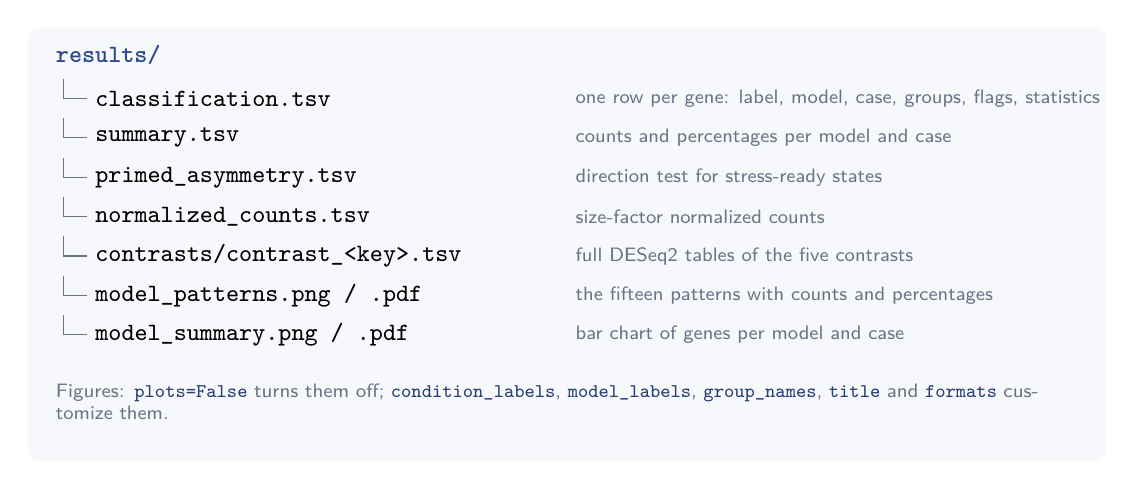
\begin{tikzpicture}[font=\ttfamily\small, every node/.style={anchor=west, inner sep=1.5pt}]
  \fill[codebg, rounded corners=4pt] (-0.3,0.45) rectangle (13.4,-5.05);
  \node at (0,0.1) {\textbf{\color{navy}results/}};
  \foreach \y/\f/\d in {
      {-0.45}/{classification.tsv}/{one row per gene: label, model, case, groups, flags, statistics},
      {-0.95}/{summary.tsv}/{counts and percentages per model and case},
      {-1.45}/{primed\_asymmetry.tsv}/{direction test for stress-ready states},
      {-1.95}/{normalized\_counts.tsv}/{size-factor normalized counts},
      {-2.45}/{contrasts/contrast\_<key>.tsv}/{full DESeq2 tables of the five contrasts},
      {-2.95}/{model\_patterns.png / .pdf}/{the fifteen patterns with counts and percentages},
      {-3.45}/{model\_summary.png / .pdf}/{bar chart of genes per model and case}}
    { \draw[muted] (0.15,\y+0.25) |- (0.45,\y);
      \node at (0.5,\y) {\f};
      \node[font=\sffamily\scriptsize, text=muted] at (6.6,\y) {\d}; }
  \node[font=\sffamily\scriptsize, text=muted, text width=12.6cm] at (0,-4.3)
    {Figures: \code{plots=False} turns them off; \code{condition\_labels}, \code{model\_labels},
     \code{group\_names}, \code{title} and \code{formats} customize them.};
\end{tikzpicture}
\caption{Contents of the results folder.}
\label{fig:files}
\end{figure}

\subsection{The classification table}

\begin{center}
\small
\begin{tabularx}{\linewidth}{>{\ttfamily\color{navy!85!black}}l Y}
\toprule
\textsf{\textbf{column}} & \textsf{\textbf{content}}\\
\midrule
label & e.g. \code{stress\_ready\_3}\\
model, case & the two parts of the label\\
primed\_group & group whose control level equals the other's stressed level (stress-ready only)\\
responding\_group & A, B, \code{both} or \code{none} (with your group names)\\
description & a readable sentence, e.g. ``PL12 is induced under stress up to the control level of IL22''\\
flags & \code{na\_treated\_as\_not\_de}, \code{basal\_difference\_not\_significant}\\
<key>\_log2FoldChange, <key>\_padj & statistics of the five contrasts\\
\bottomrule
\end{tabularx}
\end{center}

\subsection{Summaries and denominators}

\code{summary} reports two percentages on purpose: \code{pct\_of\_responsive} uses the genes that respond
in at least one group, and \code{pct\_of\_all} uses every classified gene. Mixing the two denominators is
a common source of confusion when reporting results.

\code{primed\_asymmetry()} asks whether one group is \emph{more often} primed. A larger raw number of
stress-ready genes in one direction can simply mean that one group has more responsive genes; the test
compares the \emph{fraction} of single-group responses that end in a stress-ready state, with Fisher's
exact test.

\subsection{Figures}

Two figures are written next to the tables: \code{model\_summary}, a bar chart of genes per model
and case, and \code{model\_patterns}, the fifteen patterns annotated with counts and percentages.

\begin{figure}[H]
\centering
\begin{minipage}[c]{0.47\linewidth}
  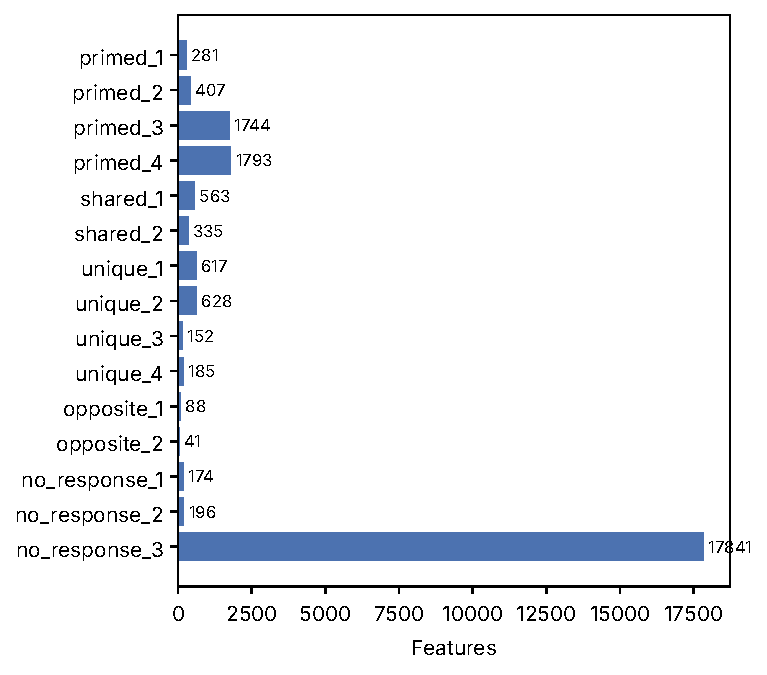
\includegraphics[width=\linewidth]{figures/rice_summary.pdf}
\end{minipage}\hfill
\begin{minipage}[c]{0.48\linewidth}\small
\textbf{\sffamily model\_summary} -- genes per model and case (left, rice example).\\[6pt]
\textbf{\sffamily model\_patterns} -- the fifteen patterns annotated with counts and percentages
(Figures~\ref{fig:rice} and \ref{fig:ovarian}).\\[6pt]
Customize them:
\begin{lstlisting}[style=py, basicstyle=\ttfamily\scriptsize]
res.save("results",
  condition_labels=("Ctrl", "NaCl"),
  model_labels={"stress_ready": "Primed"},
  formats=("png",))
\end{lstlisting}
\end{minipage}
\caption{Bar chart written as \code{model\_summary.png/pdf}.}
\end{figure}

% ================================================================== 9
\section{Worked examples}
\label{sec:examples}

Both data sets are bundled with the package and come from raw counts deposited by the authors in GEO;
no read alignment is needed. The numbers below come from the R/DESeq2 run.

\begin{center}
\small
\begin{tabularx}{\linewidth}{>{\ttfamily}l Y Y c}
\toprule
\textsf{\textbf{name}} & \textsf{\textbf{groups (A vs B)}} & \textsf{\textbf{conditions}} & \textsf{\textbf{size}}\\
\midrule
rice\_salt & PL12 (salt-sensitive) vs IL22 (\emph{Saltol} introgression line) & control vs 24 h 80 mM NaCl & 36\,844 \(\times\) 12\\
ovarian\_brequinar & OVCAR5 cisplatin-sensitive vs cisplatin-resistant & vehicle vs brequinar & 59\,453 \(\times\) 12\\
\bottomrule
\end{tabularx}
\end{center}

\subsection{Plant: rice under salt stress (GEO GSE167342)}

Leaves of the salt-sensitive \emph{japonica} cultivar \textcolor{grpA}{\textbf{PL12}} (A) and the
salt-tolerant introgression line \textcolor{grpB}{\textbf{IL22}} (B; FL478 \(\times\) PL12, carrying the
\emph{Saltol} QTL), control vs 24 h of 80 mM NaCl, 3 replicates. Columns S40--S72 of the count matrix
are the authors' library names; the bundled sample table links each one to its GEO sample.

\begin{shcode}
cd examples/rice_salt_GSE167342
python run_python.py        # or: Rscript run_r.R
\end{shcode}

\begin{figure}[htbp]
\centering
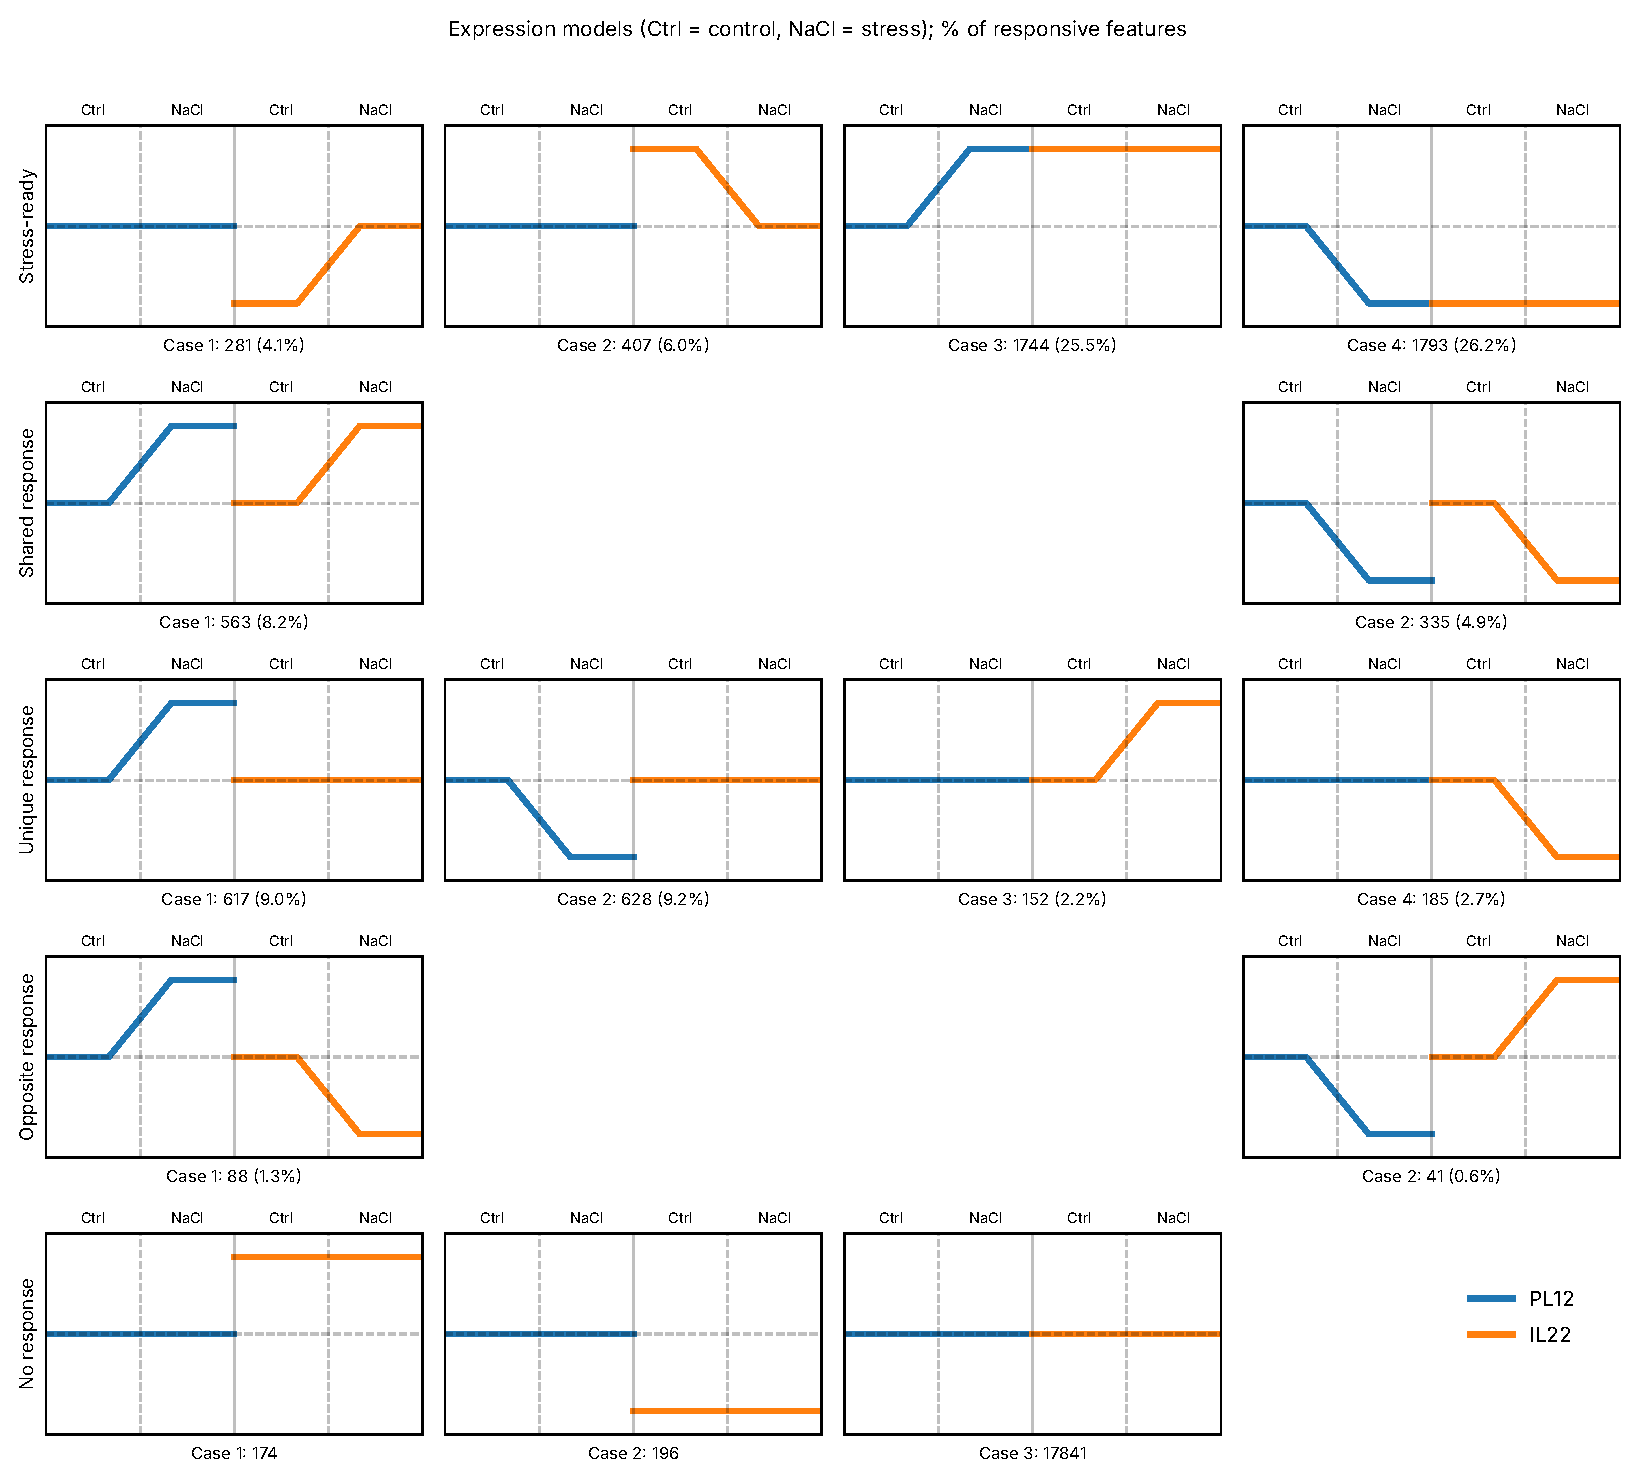
\includegraphics[width=0.9\linewidth]{figures/rice_patterns.pdf}
\caption{Rice example, \code{paper} preset (Ctrl = control, NaCl = salt). 25\,045 genes after filtering.}
\label{fig:rice}
\end{figure}

\begin{table}[htbp]
\centering\small
\caption{Rice: number of genes per model under the two presets.}
\begin{tabular}{l r r}
\toprule
\textsf{\textbf{model}} & \textsf{\textbf{paper}} & \textsf{\textbf{strict}}\\
\midrule
stress-ready 1 / 2 / 3 / 4 & 281 / 407 / 1\,744 / 1\,793 & 35 / 72 / 297 / 189\\
shared 1 / 2 & 563 / 335 & 563 / 335\\
unique 1 / 2 / 3 / 4 & 617 / 628 / 152 / 185 & 2\,024 / 2\,180 / 389 / 514\\
opposite 1 / 2 & 88 / 41 & 88 / 41\\
no response 1 / 2 / 3 & 174 / 196 / 17\,841 & 174 / 196 / 13\,587\\
unclassified & 0 & 4\,361\\
\bottomrule
\end{tabular}
\end{table}

\textbf{What it shows.}
\begin{itemize}
  \item The sensitive line reacts much more: 4\,782 single-line responses in PL12 against 1\,025 in IL22,
        consistent with IL22 experiencing less stress.
  \item The lines are nearly isogenic, so basal differences are rare (370 non-responsive genes). Under
        the \code{paper} rules 62\% of the responsive genes are called stress-ready, mostly because a gene
        that responds in one line is ``not significantly different'' from the unchanged level of the other.
        Requiring a basal difference keeps 593 of 4\,225.
  \item The apparent asymmetry (74.0\% vs 67.1\%, \(p=1.2\times10^{-5}\)) disappears under \code{strict}
        (10.4\% vs 10.6\%, \(p=0.82\)).
\end{itemize}

\subsection{Human: ovarian cancer cells and brequinar (GEO GSE283381)}

OVCAR5 high-grade serous ovarian cancer cells: the cisplatin-sensitive parental line
\textcolor{grpA}{\textbf{CisS}} (A) and a cisplatin-resistant derivative \textcolor{grpB}{\textbf{CisR}} (B),
treated with vehicle or \textbf{brequinar}, an inhibitor of DHODH and therefore of \emph{de novo}
pyrimidine synthesis, 3 replicates. The raw HTSeq counts deposited by the authors (one file per sample)
were merged into one matrix without any transformation.

\begin{figure}[htbp]
\centering
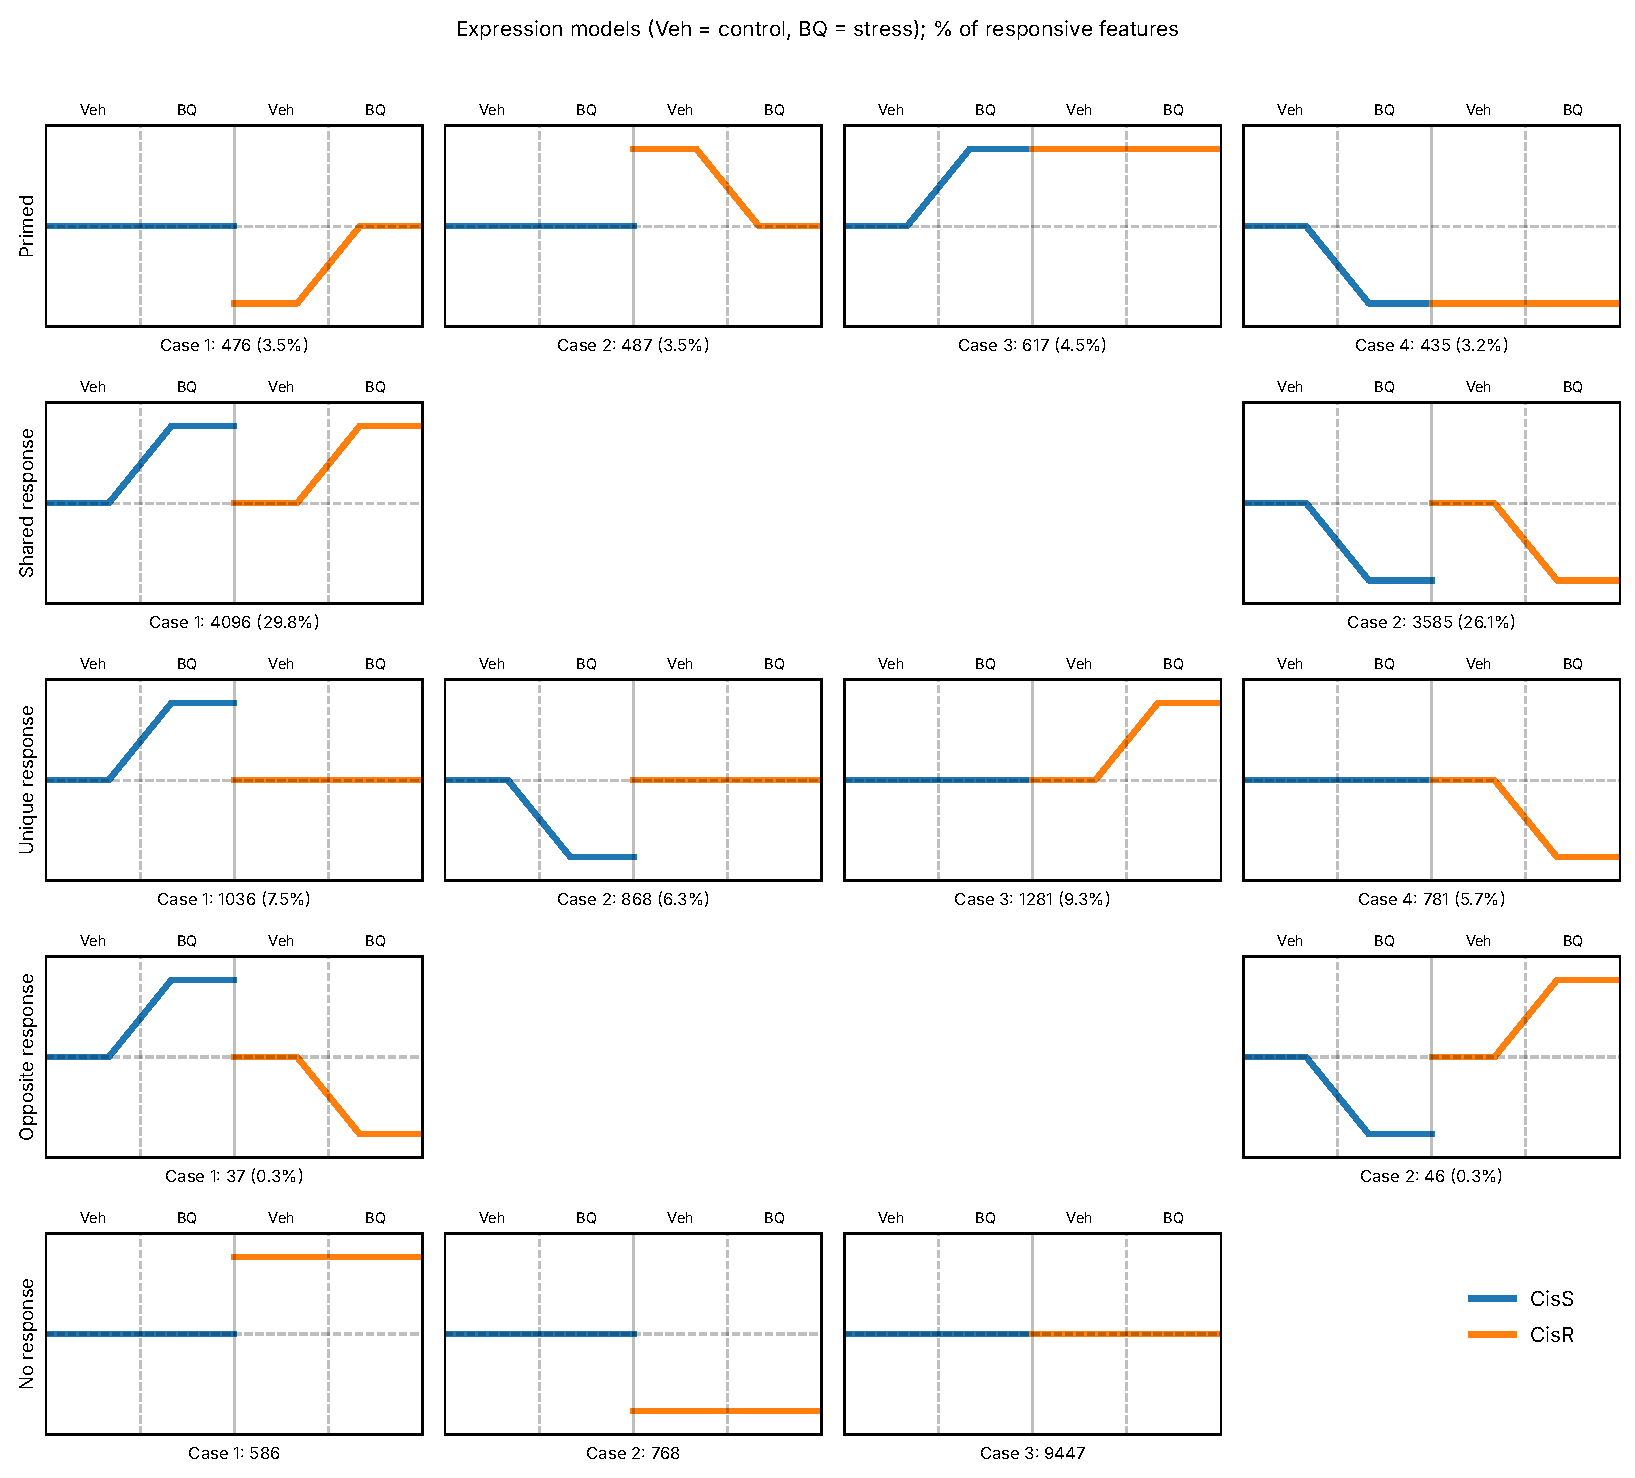
\includegraphics[width=0.9\linewidth]{figures/ovarian_patterns.pdf}
\caption{Ovarian example, \code{paper} preset (Veh = vehicle, BQ = brequinar). 24\,546 genes after filtering.}
\label{fig:ovarian}
\end{figure}

\begin{figure}[htbp]
\centering
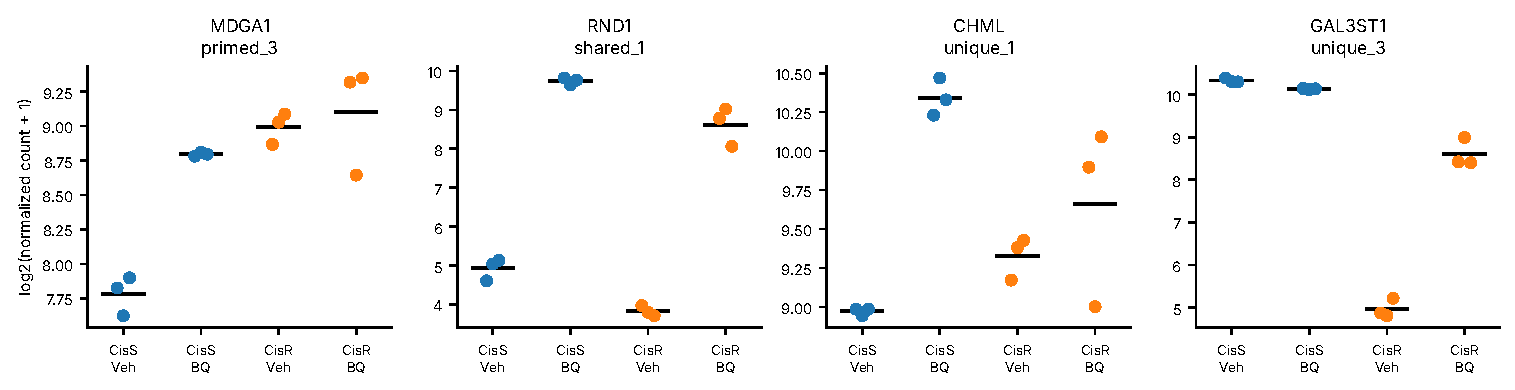
\includegraphics[width=\linewidth]{figures/ovarian_genes.pdf}
\caption{Real genes from the ovarian example, one per model (normalized counts; dots are replicates,
bars are means). \textsf{MDGA1}: induced by brequinar in the sensitive cells up to the constitutive level of
the resistant cells (stress-ready 3, \code{strict} preset).}
\label{fig:genes}
\end{figure}

\begin{table}[htbp]
\centering\small
\caption{Ovarian cells: number of genes per model under the two presets.}
\begin{tabular}{l r r}
\toprule
\textsf{\textbf{model}} & \textsf{\textbf{paper}} & \textsf{\textbf{strict}}\\
\midrule
stress-ready 1 / 2 / 3 / 4 & 476 / 487 / 617 / 435 & 162 / 179 / 159 / 146\\
shared 1 / 2 & 4\,096 / 3\,585 & 4\,096 / 3\,585\\
unique 1 / 2 / 3 / 4 & 1\,036 / 868 / 1\,281 / 781 & 1\,409 / 1\,123 / 1\,568 / 1\,072\\
opposite 1 / 2 & 37 / 46 & 37 / 46\\
no response 1 / 2 / 3 & 586 / 768 / 9\,447 & 586 / 768 / 6\,755\\
unclassified & 0 & 2\,855\\
\bottomrule
\end{tabular}
\end{table}

\textbf{What it shows.}
\begin{itemize}
  \item Brequinar changes many genes in both lines: most responsive genes are shared (7\,681 of 13\,745).
  \item The two cell lines differ at basal level for many genes, so \code{strict} keeps about a third of
        the stress-ready calls (646 of 2\,015), compared with one in seven in rice.
  \item Neither line is globally more primed: 35.6\% vs 31.8\% under \code{paper} (\(p=0.002\)) and
        10.8\% vs 11.4\% under \code{strict} (\(p=0.43\)).
\end{itemize}

% ================================================================== 10
\section{Interpreting results}
\label{sec:interpret}

\begin{figure}[htbp]
\centering
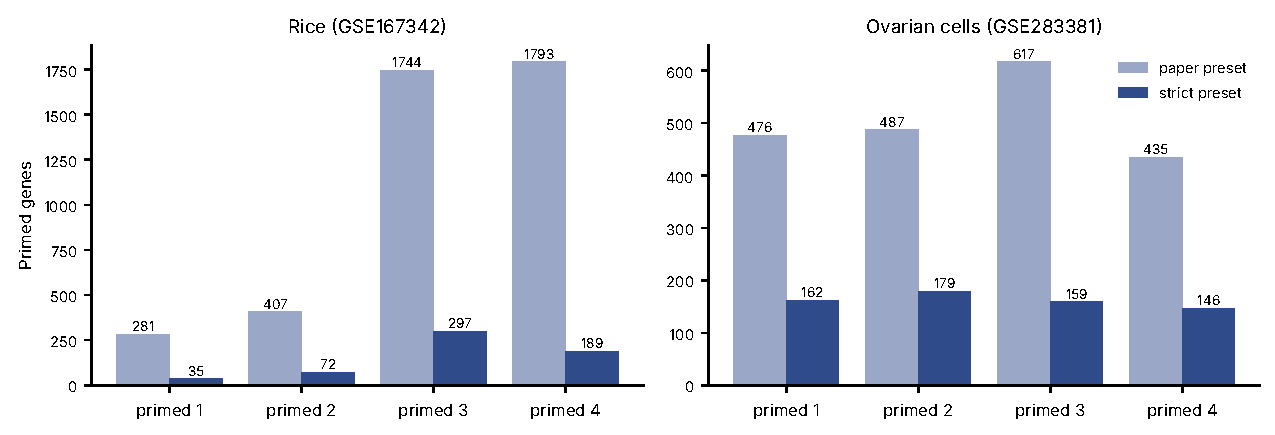
\includegraphics[width=0.95\linewidth]{figures/paper_vs_strict.pdf}
\caption{Stress-ready genes under the two presets. The reduction is strongest when the groups have few
basal differences (rice).}
\label{fig:pvs}
\end{figure}

\begin{figure}[htbp]
\centering
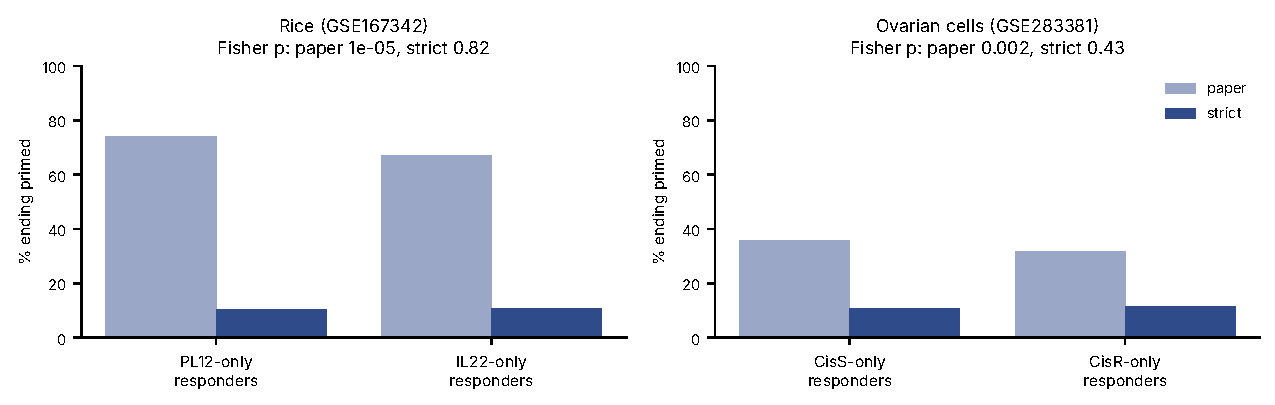
\includegraphics[width=0.95\linewidth]{figures/asymmetry.pdf}
\caption{Fraction of single-group responses that end in a stress-ready state. Under the \code{paper}
rules a small asymmetry appears in both data sets; under \code{strict} it disappears.}
\label{fig:asym}
\end{figure}

\begin{itemize}
  \item \textbf{False positives flow into stress-ready.} A false-positive response in one group, for a gene
        whose basal level does not differ between groups, is classified as stress-ready under the
        \code{paper} rules. \code{require\_basal\_difference} blocks this route.
  \item \textbf{Unique vs shared.} ``Significant in A and not in B'' does not prove that the responses
        differ. If the difference of responses is your question, test the interaction
        (\code{\textasciitilde{} group + group:condition}) separately.
  \item \textbf{Directional claims.} Use \code{primed\_asymmetry()} before concluding that one group is
        more pre-adapted.
  \item \textbf{Equal stress?} The same treatment may be perceived differently by the two groups; fewer
        responses in one group can mean less perceived stress rather than pre-adaptation.
  \item \textbf{Replicates.} At least 3 per cell; with 2, results are exploratory.
\end{itemize}

% ================================================================== 11
\section{Cross-species analyses}

When the two groups are different species, each gene must be paired with its ortholog first.

\begin{enumerate}
  \item Quantify each species against its own reference to obtain raw gene-level counts.
  \item Define one-to-one orthologs, for example as reciprocal best BLASTp hits:
\begin{shcode}
makeblastdb -in B.faa -dbtype prot -out B
makeblastdb -in A.faa -dbtype prot -out A
blastp -query A.faa -db B -outfmt 6 -evalue 1e-5 -max_target_seqs 5 > A_vs_B.tsv
blastp -query B.faa -db A -outfmt 6 -evalue 1e-5 -max_target_seqs 5 > B_vs_A.tsv
\end{shcode}
  \item Build the ortholog table and merge the two count matrices:
\begin{pycode}
orth = orr.reciprocal_best_hits("A_vs_B.tsv", "B_vs_A.tsv",
                                strip_pattern=r"\.\d+$")
counts = orr.merge_ortholog_counts(counts_a, counts_b, orth)
res = orr.run_orthoresponse(
    counts, samples, group_col="species", condition_col="treatment",
    group_a="S_lycopersicum", group_b="S_pennellii",
    control="control", stress="drought")
\end{pycode}
\end{enumerate}

Any other one-to-one ortholog table (OrthoFinder single-copy orthogroups, Ensembl Compara, PLAZA)
works as long as it has one column per species. \code{length\_normalize=True} applies the length
correction \(Q=\mathrm{round}(E/L_{\mathrm{kb}})\) of the original tomato study; use it to replicate that
analysis or as a sensitivity check. Remember that basal differences between species mix biology with
technical effects such as reference quality, transcript length and annotation.

% ================================================================== 12
\section{Python and R}

\begin{itemize}
  \item \textbf{Classifier: identical.} Given the same contrast tables, both languages return the same
        label for every feature. This was verified on 240\,000 random classifications with four option
        sets, on a shared fixture used by both test suites, and on both worked examples.
  \item \textbf{Differential-expression engine: very close.} DESeq2 and PyDESeq2 are separate
        implementations. Fold changes agree almost perfectly (correlation \(>0.9999\)), but adjusted
        p-values near the threshold can differ: 99.5\% of labels agreed on the rice example and 96.3\% on
        the ovarian one.
\end{itemize}

\begin{tip}[Exact agreement across languages]
Compute the contrasts once (e.g. in R), write them with \code{write\_contrasts()}, and classify the same
tables in either language.
\end{tip}

% ================================================================== 13
\section{Function reference}

\begin{center}
\small
\begin{tabularx}{\linewidth}{>{\ttfamily\color{grpA!85!black}}l >{\ttfamily\color{grpB!85!black}}l Y}
\toprule
\textsf{\textbf{Python}} & \textsf{\textbf{R}} & \textsf{\textbf{purpose}}\\
\midrule
run\_orthoresponse() & orthoresponse() & counts \(\rightarrow\) contrasts \(\rightarrow\) classification\\
run\_contrasts() & run\_contrasts() & DESeq2 / PyDESeq2 fit and the five contrasts\\
build\_design() & build\_design() & map samples to the four cells\\
classify\_responses() & classify\_responses() & the decision tree\\
classification\_options() & classification\_options() & presets and options\\
model\_definitions() & model\_definitions() & table of models and cases\\
summarize\_classification() & summarize\_classification() & counts and percentages\\
primed\_asymmetry() & primed\_asymmetry() & direction test for stress-ready states\\
equivalence\_test() & equivalence\_test() & TOST for log2 fold changes\\
read\_contrasts() / write\_contrasts() & {\color{grpB!85!black}same} & contrast tables from / to files\\
reciprocal\_best\_hits() & reciprocal\_best\_hits() & orthologs from two BLAST files\\
merge\_ortholog\_counts() & merge\_ortholog\_counts() & ortholog-level count matrix\\
plotting.plot\_model\_patterns() & plot\_model\_patterns() & the fifteen patterns with counts\\
plotting.plot\_summary() & plot\_summary() & bar chart of models\\
save\_plots() & save\_plots() & write both figures\\
OrthoResponseResult.save() & save\_orthoresponse() & write all outputs, including figures\\
load\_example() & load\_example() & bundled data (\code{rice\_salt}, \code{ovarian\_brequinar})\\
example\_files() / export\_example() & {\color{grpB!85!black}same} & paths / copies of the example files\\
\bottomrule
\end{tabularx}
\end{center}
Every function is documented in place. In Python use, for example,
\code{help(orr.classify\_responses)}; in R, \code{?classify\_responses}.

% ================================================================== 14
\section{Troubleshooting}

\begin{center}
\small
\begin{tabularx}{\linewidth}{>{\raggedright\arraybackslash}p{5.2cm} Y}
\toprule
\textsf{\textbf{message}} & \textsf{\textbf{cause and fix}}\\
\midrule
\emph{Empty design cell(s)} & \code{group\_a}, \code{group\_b}, \code{control} and \code{stress} do not match
the values of the sample table (they are case-sensitive).\\
\emph{Expected N fields in line M} & the sample table has spaces instead of tabs; fix it or read it with
\code{sep=r"\textbackslash{}s+"}.\\
\emph{Counts are not integers} & TPM, FPKM or normalized values were given; use raw counts, or
\code{round\_counts=True} for estimated counts.\\
\emph{Samples missing from the count matrix} & sample-table row names differ from the count-matrix columns.\\
\emph{Contrast tables cover different features} & the five tables were filtered differently; only shared
features are used.\\
\emph{equivalence\_margin requires an lfcSE column} & keep the standard-error column when exporting contrasts.\\
\emph{run\_contrasts() needs PyDESeq2} & \code{pip install "orthoresponse[deseq]"}.\\
No figures in the results folder & update to version 0.4.0 or later, and install matplotlib
(\code{pip install "orthoresponse[plot]"}).\\
\bottomrule
\end{tabularx}
\end{center}

% ================================================================== 15
\section{Citation and license}

If you use \pkg{}, please cite the software using the metadata in \code{CITATION.cff}
(GitHub's \emph{Cite this repository} button). DESeq2 and PyDESeq2 should be cited as well:

\begin{itemize}
  \item Love MI, Huber W, Anders S (2014). Moderated estimation of fold change and dispersion for RNA-seq
        data with DESeq2. \emph{Genome Biology} 15: 550.
  \item Muzellec B, Telenczuk M, Cabeli V, Andreux M (2023). PyDESeq2: a python package for bulk RNA-seq
        differential expression analysis. \emph{Bioinformatics} 39: btad547.
\end{itemize}

\textbf{Data sources of the examples:} GEO GSE167342 (rice) and GEO GSE283381 (ovarian cancer cells).

\textbf{License:} MIT. \quad \textbf{Source code:}
\href{https://github.com/Cold7/orthoresponse}{github.com/Cold7/orthoresponse}

\end{document}
